\newpage
\subsection{Regression ANN: Cross-validation algorithm}\label{sec:ANN_reg_algorithm}


\begin{enumerate}
\item \textbf{Outer CV split:} We first divided the data into $\mathcal{D}^{\text{par}}$ and  $\mathcal{D}^{\text{test}}$ using hold-out. All attribute columns in $\bm{X}$ were normalized (exactly like we did in report 1: subtract mean and divide by standard deviation).

\item \textbf{Inner CV split:} We then split $\mathcal{D}^{\text{par}}$ into $K = 10$ partitions $\mathcal{D}_1^{\text{par}} \, .. \, \mathcal{D}_{10}^{\text{par}}$, used to perform K-fold cross-validation.

\item \textbf{Training:} For each K-fold partition $\mathcal{D}_k^{\text{par}}$, $k = 1 \, .. \, 10$, we trained 30 models ($H = 1 \, .. \, 30$ hidden nodes), and recorded the validation error $E_{\mathcal{M}_H, k}^{\text{val}}$, using the  sum of squared differences as the error function. This error represents how well this particular model performed in the given K-fold split. In the code, the validation error is recorded in a 2D array $\text{E(k, H)}$.

\item \textbf{Validation error:} After training, we computed the error for each model, $\hat{E}_H^{\text{gen}} = \sum_{k=1}^{10} \frac{ | \mathcal{D}_k^{\text{val}}  | }{ | \mathcal{D}^{ \text{par} } | } E_{\mathcal{M}_H, k}^{\text{val}}$. Since split the training data into 10 K-fold partitions, $\frac{ | \mathcal{D}_k^{\text{val}}  | }{ | \mathcal{D}^{ \text{par} } | } = \frac{1}{10}$. This error represents how well the model performed overall, across all K-fold splits.

\item \textbf{Choose model:} We selected the optimal model $\mathcal{M}^{*} = M_{H^{*}}$, where $H^*$ is the number of hidden nodes that lead to the smallest validation error $\hat{E}_H^{\text{gen}}$.

\item \textbf{Generalization error:} Finally, we trained the optimal model on the held-out test set $\mathcal{D}^{\text{test}}$, and estimated the generalization error $\hat{E}^{\text{gen}}$ based on this test.
\end{enumerate}

\newpage
\subsection{Regression ANN: trained network}

\begin{figure}[H]
    \centering
    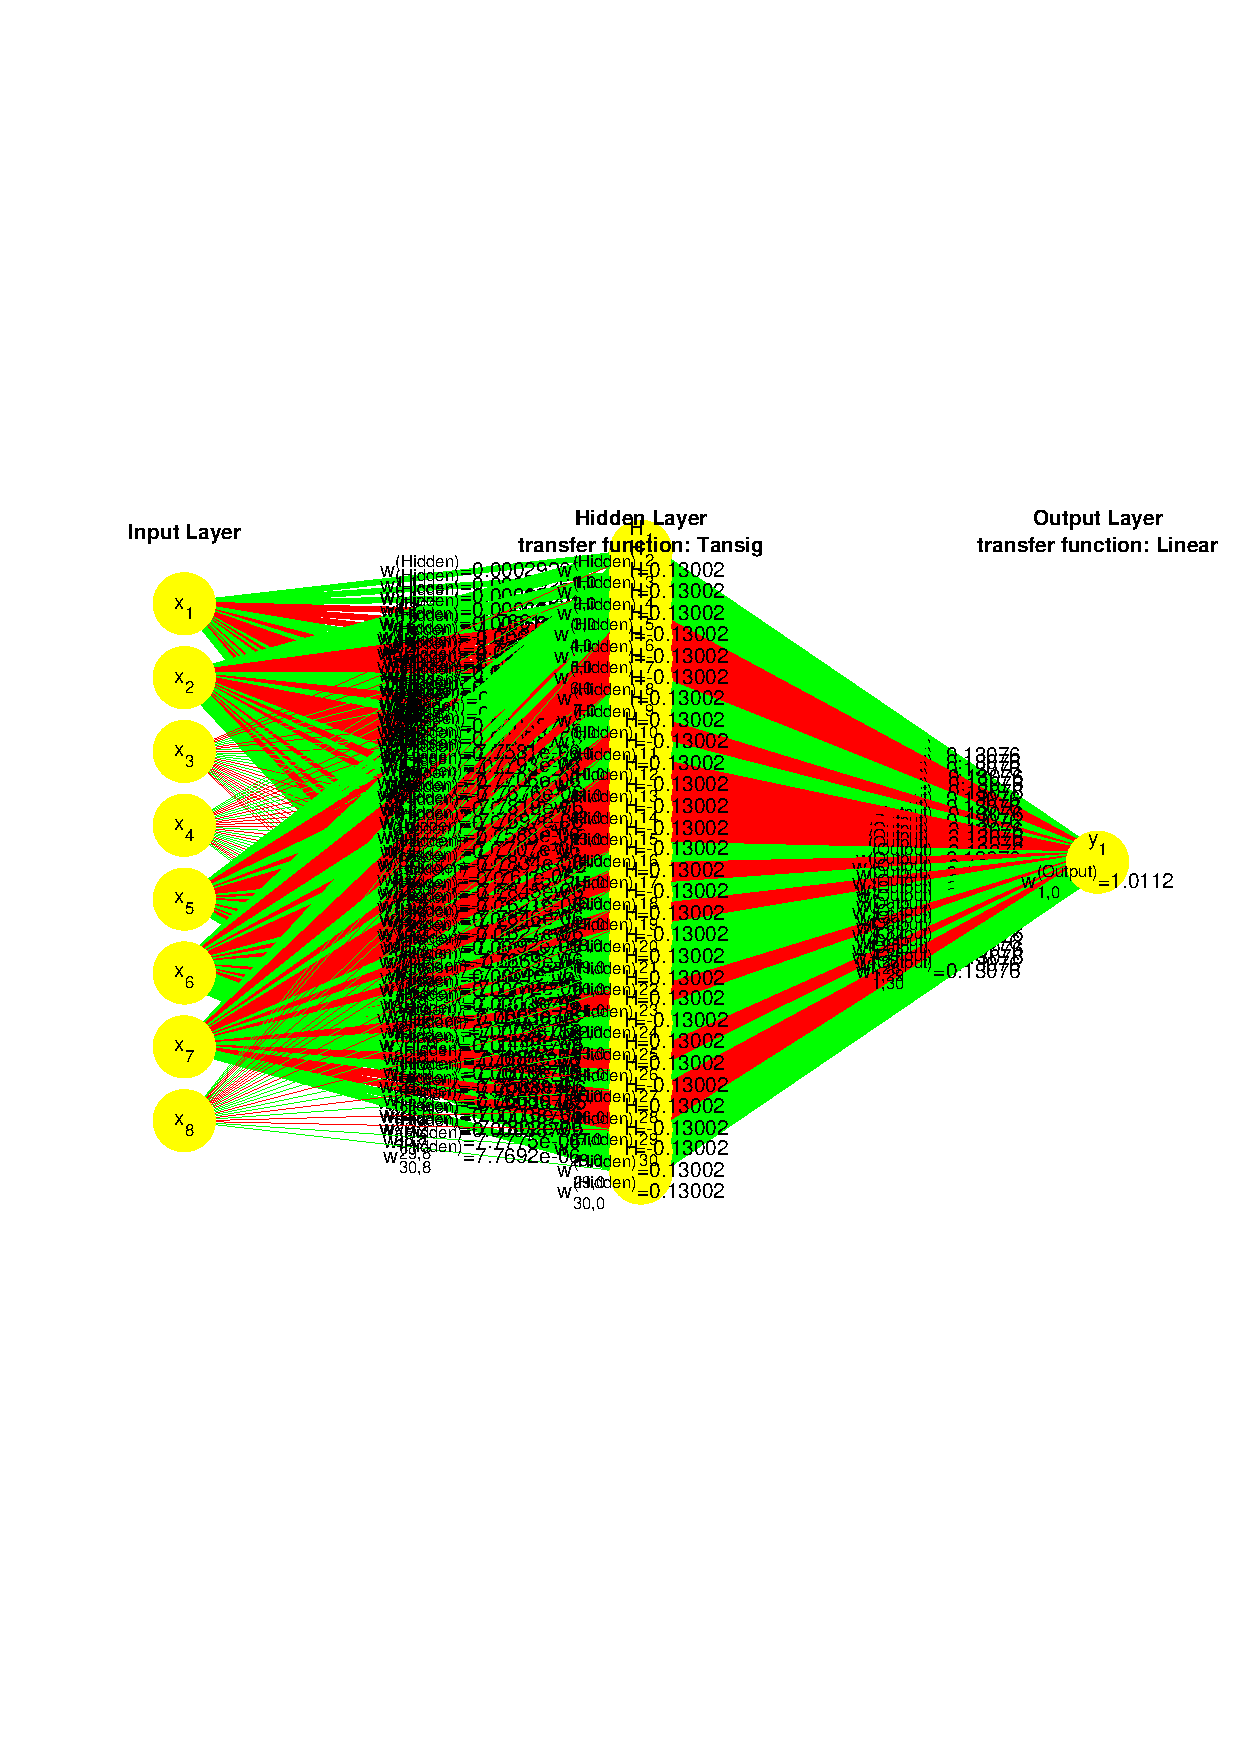
\includegraphics[width=1.0\textwidth]{fig/regression/ANN_reg_evaluating_best_model_trained_network.pdf}
    \caption{Visualization of the trained network in the ANN regression problem. We have 8 input variables (ratio weight percent attributes), so there are $D=8$ input nodes. The inner CV loop selected $H=30$ as the optimal number of hidden nodes. The goal is to predict the refraction index \texttt{RI}, a single value, so there is $D = 1$ output node. The network contains so many nodes that the neural weights become unreadable. From the line widths between nodes, however, we notice that input attributes 4 and 8 (corresponding to chemical composition components \texttt{Si} and \texttt{Fe}) have little importance on the refractive index \texttt{RI}}
\end{figure}